\documentclass[aspectratio=169,obeyspaces,spaces,hyphens,dvipsnames]{beamer}
\usepackage[utf8]{inputenc}
\usepackage{lmodern}% http://ctan.org/pkg/lm
\usepackage{hyperref}
\usepackage{xcolor}
\usepackage{pgfplots}
\usepackage{tikz}
\usepackage[normalem]{ulem}

\mode<presentation>
\usetheme{ToganLabs}

\def\signed #1{{\leavevmode\unskip\nobreak\hfil\penalty50\hskip2em
  \hbox{}\nobreak\hfil(#1)
  \parfillskip=0pt \finalhyphendemerits=0 \endgraf}}

\newsavebox\mybox
\newenvironment{aquote}[1]
  {\savebox\mybox{#1}\begin{quotation}}
  {\signed{\usebox\mybox}\end{quotation}}

\title{Getting started with Buildroot}
\authors{Trevor Woerner}
\email{trevor@toganlabs.com}
\slidesurl{https://cm.e-ale.org/2019/SCaLE17x/buildroot}
\institute{Togán Labs}
\conference{SCaLE 17x}

\begin{document}

\addtocontents{toc}{\protect\setcounter{tocdepth}{-1}}
\section{Getting started with Buildroot}
\addtocontents{toc}{\protect\setcounter{tocdepth}{2}}

\begin{frame}{Trevor Woerner}
  \begin{columns}
    \column{0.7\textwidth}
      \begin{itemize}
      \item Senior Software Developer at Togán Labs
        \begin{itemize}
        \item Embedded Linux Development and Consulting
        \item Specialize in {\bf OpenEmbedded/Yocto}
        \item Strong open-source focus
        \end{itemize}
      \end{itemize}
    \column{0.3\textwidth}
      
\includegraphics[width=\textwidth]{toganlabs/toganlabs-full.pdf}
    \end{columns}
\end{frame}

\begin{frame}{Thomas Petazzoni}
  \begin{columns}
    \column{0.7\textwidth}
      \begin{itemize}
      \item Initially created this presentation
      \item CTO and Embedded Linux engineer at Bootlin
      \item {\bf major} contributor to buildroot
      \begin{itemize}
        \item one of 3 people with commit access to buildroot
      \end{itemize}
      \item Strong open-source focus
      \end{itemize}
    \column{0.3\textwidth}
      \includegraphics[width=\textwidth]{bootlin/logo-square.pdf}
    \end{columns}
\end{frame}

\begin{frame}{Using an embedded Linux system}
  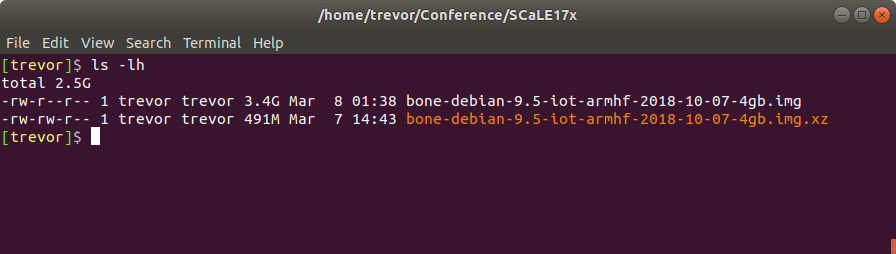
\includegraphics[width=\textwidth]{woerner/imgsize.png}
  \vspace{0.1cm}
  \begin{itemize}
    \item the first thing you did at the very start of the labs
    \item has allowed you to do everything you've done with the board
    \item wrote one {\bf HUGE} image to the SDcard -- \textit{3.4GB}!!
    \item it took my laptop over 13 minutes
  \end{itemize}
\end{frame}

\begin{frame}{Using an embedded Linux system}
  \begin{itemize}
    \item what does the SDcard look like post-flashing?
  \end{itemize}
  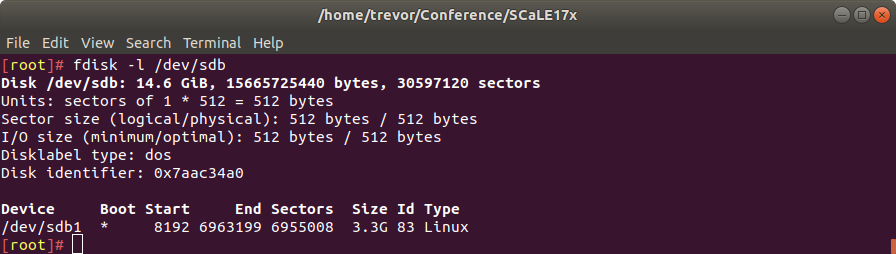
\includegraphics[width=\textwidth]{woerner/fdisk.png}
\end{frame}

\begin{frame}{Using an embedded Linux system}
  \begin{itemize}
    \item one big file was flashed, but the card now has partitions and lots of files
    \item works cross-platform (x86\_64 host, ARM target)
  \end{itemize}
  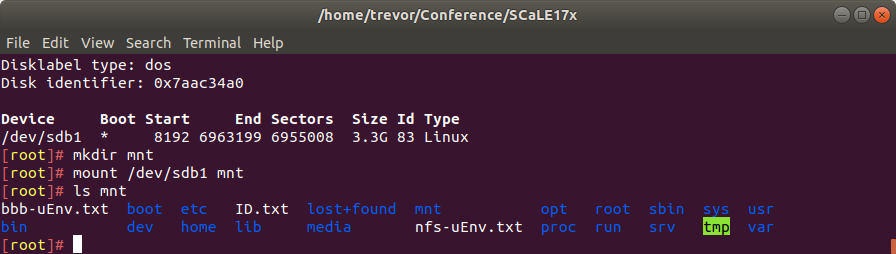
\includegraphics[width=\textwidth]{woerner/mount-sd.png}
\end{frame}

\begin{frame}{Using an embedded Linux system}
  \begin{itemize}
    \item it's all there in the \texttt{*.img} file
  \end{itemize}
  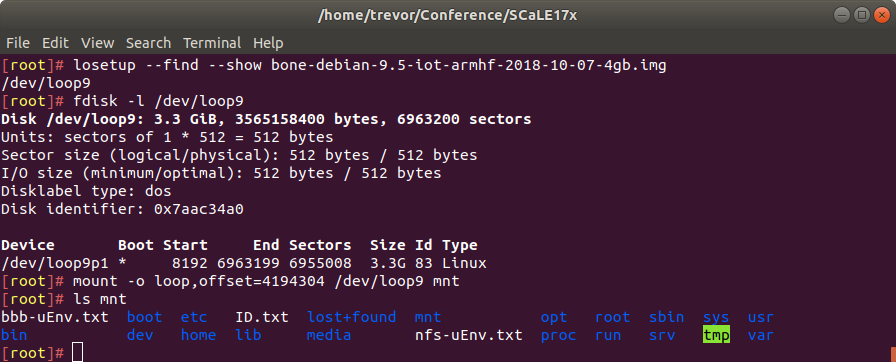
\includegraphics[width=\textwidth]{woerner/mount-file.png}
\end{frame}

\begin{frame}{Using an embedded Linux system}
  \begin{itemize}
    \item it's all there in the \texttt{*.img} file
  \end{itemize}
  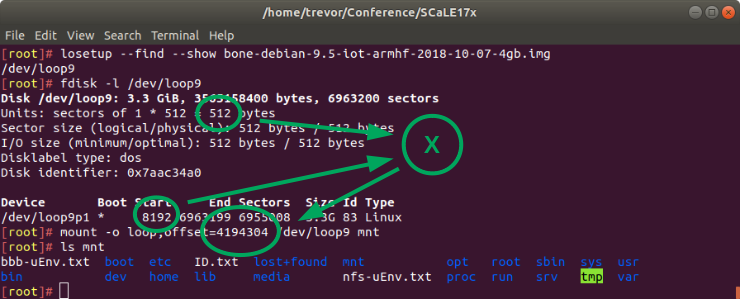
\includegraphics[width=\textwidth]{woerner/mount-file-circle.png}
\end{frame}

\begin{frame}{Can I build an embedded Linux system?}
  \begin{itemize}
    \item with my own contents
    \begin{itemize}
      \item bootloader
      \item kernel
      \item init
      \item apps ($\rightarrow$ dependencies)
    \end{itemize}
    \item to target multiple devices
    \item within a certain size (smaller)
    \item containing only what a production device needs
    \item with the latest fixes
    \item built up from nothing, not simply imaging a disk (horse/cart)
  \end{itemize}
\end{frame}

\begin{frame}{Can I build an embedded Linux system?}
  \begin{center}
    \huge YES!
  \end{center}
\end{frame}

\begin{frame}{Can I build an embedded Linux system?}
  Caveats:
  \begin{itemize}
    \item cross-compiling/toolchain
    \item find/get the sources (bzr, cvs, git, hg, scp, svn, wget, ...) can't hope for pre-compiled
    \item checksum (md5, sha256, sha512, ...)
    \item dependencies
    \item unpack (gzip, bzip2, xz, zip, ...)
    \item patch
    \item configure
    \item build (make, cmake, ant, maven, waf, ninja, gyp, meson, ...)
    \item device-specific tweaks/tricks
    \item lots of choice, hard to get right
    \item one doesn't slap together a cohesive, working set, by accident
  \end{itemize}
\end{frame}

\begin{frame}{Can I build an embedded Linux system?}
  problems:
  \begin{itemize}
    \item there is no "{\bf one correct way}" to write (open-source) software
    \begin{itemize}
      \item language
      \item repository system
      \item build system
      \item location
      \item licensing
    \end{itemize}
    \item not enough developers consider cross-compilation
  \end{itemize}
  solution:
  \begin{itemize}
    \item use an embedded Linux build system
    \item {\bf PLEASE} don't "roll your own"
  \end{itemize}
\end{frame}

\begin{frame}{Building an embedded Linux system}
  \begin{center}
    \uncover<1>{\includegraphics[width=0.2\textwidth]{build-solutions-distros.pdf}}
    \uncover<3>{\includegraphics[width=0.2\textwidth]{build-solutions-build-systems.pdf}}
    \uncover<2>{\includegraphics[width=0.2\textwidth]{build-solutions-hand-made.pdf}}
  \end{center}
  \only<1>{
    \begin{itemize}
    \item[+] Readily available
    \item[-] Large, usually 100+ MB ($\rightarrow$ GB!)
    \item[-] Not available for all architectures/devices
    \item[-] Not easy to customize
    \item[-] Generally require native compilation
    \end{itemize}
  }
  \only<2>{
    \begin{itemize}
    \item[+] Smaller and flexible
    \item[-] Very hard to handle cross-compilation and dependencies
    \item[-] Not reproducible
    \item[-] No benefit from other people's work
    \end{itemize}
  }
  \only<3>{
    \begin{itemize}
    \item[+] Small and flexible
    \item[+] Reproducible, handles cross-compilation and dependencies
    \item[+] Available for virtually all architectures
    \item[-] One tool to learn
    \item[-] Build time
    \end{itemize}
  }
\end{frame}

\begin{frame}{Embedded Linux build system: principle}
  \begin{center}
    \includegraphics[width=0.9\textwidth]{buildsystem-principle.pdf}
  \end{center}
  \begin{itemize}[<+->]
  \item Building from source $\rightarrow$ lot of flexibility
  \item Cross-compilation $\rightarrow$ leveraging fast build machines
  \item {\bf Recipes} for building components $\rightarrow$ easy
  \end{itemize}
\end{frame}

\begin{frame}{Recipes, meta-data}
  \begin{itemize}
    \item all embedded Linux build systems have:
    \begin{itemize}
      \item a tool for building the image (i.e. \texttt{make})
      \item the {\bf recipes} or {\bf meta-data} describing how to handle each component
      \begin{itemize}
        \item where it's located (github, gitlab, bitbucket, ...)
        \item how to fetch it (wget, svn, git, ...)
        \item patches
        \item how to build (make, meson, cmake, ...)
      \end{itemize}
      \item configuration
    \end{itemize}
  \end{itemize}
\end{frame}

\begin{frame}{Buildroot at a glance}
  \begin{columns}
    \column{0.8\textwidth}
  \begin{itemize}
  \item Is an {\bf embedded Linux build system}, builds from source:
    \begin{itemize}
    \item cross-compilation toolchain
    \item root filesystem with many libraries/applications, cross-built
    \item kernel and bootloader images
    \end{itemize}
  \item {\bf Fast}, simple root filesystem in minutes
  \item {\bf Easy} to use and understand: kconfig and make
  \item {\bf Small} root filesystem, default 2 MB
  \item Roughly {\bf 2170 packages} available
  \item Generates filesystem images, not a distribution
  \item Vendor neutral
  \item Active community, stable releases every 3 months
  \item Started in 2001, oldest still maintained build system
  \item \url{http://buildroot.org}
  \end{itemize}
  \column{0.2\textwidth}
  
\includegraphics[width=\textwidth]{logo.png}
\end{columns}
\end{frame}

\begin{frame}[fragile]{Getting started}
  \begin{block}{}
    \begin{verbatim}
$ git clone git://git.busybox.net/buildroot
$ cd buildroot
$ make menuconfig
\end{verbatim}
  \end{block}
  \vspace{0.1cm}
  \begin{center}
    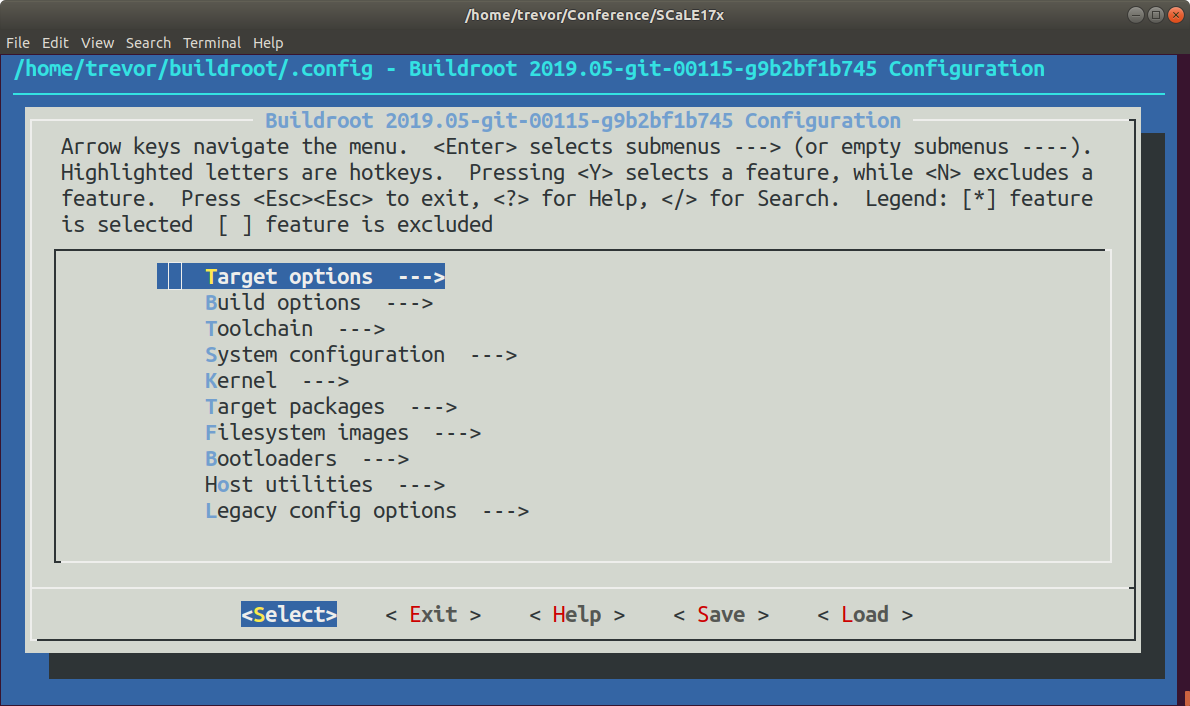
\includegraphics[width=0.6\textwidth]{woerner/buildroot-screenshot.png}
  \end{center}
\end{frame}

\begin{frame}{Buildroot configuration}
  \begin{columns}
    \column{0.4\textwidth}
    \begin{enumerate}[<+-| alert@+>]
    \item Target architecture
    \item Build options
    \item Toolchain
    \item System configuration
    \item Kernel
    \item Target packages
    \item Filesystem images
    \item Bootloaders
    \item Host utilities
    \end{enumerate}
    \column{0.6\textwidth}
    \only<1>{
      \begin{itemize}
      \item Architecture\\
        {\small ARC, ARM, Aarch64, csky, m68k, Microblaze,
          MIPS(64), NIOS II, OpenRISC, PowerPC(64), RISC-V,
          SuperH, SPARC(64), x86, x86\_64, Xtensa}
      \item Specific processor (variant) / Floating-point strategy
      \item ABI
      \end{itemize}
    }
    \only<2>{
      \begin{itemize}
      \item Download directory
      \item Number of parallel jobs
      \item Use of {\em ccache}
      \item Shared or static libraries
      \item etc.
      \end{itemize}
    }
    \only<3>{
      \begin{itemize}
      \item Buildroot toolchain
        \begin{itemize}
        \item Buildroot builds the toolchain
        \item uClibc-ng, glibc, musl
        \end{itemize}
      \item External toolchain
        \begin{itemize}
        \item Uses a pre-built toolchain
        \item Profiles for existing popular toolchains\\
          {\small Linaro, Sourcery CodeBench, etc.}
        \item Custom toolchains
        \end{itemize}
      \end{itemize}
    }
    \only<4>{
      \begin{itemize}
      \item Init system to use: Busybox, Sysvinit, Systemd
      \item \code{/dev} management solution: static, devtmpfs, mdev, udev
      \item Hostname, password, getty terminal, etc.
      \item Root filesystem overlay
      \item Custom post build and post image scripts
      \item etc.
      \end{itemize}
    }
    \only<5>{
      \begin{itemize}
      \item Kernel source (stable version, Git tree, patches)
      \item Kernel configuration
      \item Support for kernel extensions: RTAI, Xenomai, aufs, etc.
      \end{itemize}
    }
    \only<6>{
      \begin{itemize}
      \item Roughly 2170 packages
      \item Qt5, X.org, Gtk, EFL
      \item GStreamer, ffmpeg
      \item Python, Perl, Ruby, Lua, Erlang
      \item Samba, OpenSSL, OpenSSH, dropbear, lighttpd
      \item OpenGL support for various platforms
      \item And many, many more libraries and utilities
      \end{itemize}
    }
    \only<7>{
      \begin{itemize}
      \item Major filesystem formats supported
        \begin{itemize}
          \item axfs
          \item btrfs
          \item cloop
          \item cpio, for kernel initramfs
          \item cramfs
          \item ext2/3/4
          \item f2fs
          \item jffs2
          \item romfs
          \item squashfs
          \item tar
          \item ubifs
          \item yaffs2
        \end{itemize}
      \end{itemize}
    }
    \only<8>{
      \begin{itemize}
      \item Barebox
      \item Gummiboot
      \item Grub2
      \item shim
      \item Syslinux
      \item U-Boot
      \item and more platform-specific bootloaders: imx-bootlets,
        at91bootstrap, etc.
      \end{itemize}
    }
    \only<9>{
      \begin{itemize}
      \item Allows to build some native tools, useful for development.
      \end{itemize}
    }
  \end{columns}
\end{frame}

\begin{frame}{Building and using}
  \begin{itemize}
  \item To start the build: \code{make}
  \item Results in \code{output/images}:
    \begin{itemize}
    \item \code{rootfs.ext4}, root filesystem in ext4 format
    \item \code{zImage}, Linux kernel image
    \item \code{am335x-pocketbeagle.dtb}, Linux kernel Device Tree
      blob
    \item \code{u-boot.img}, U-Boot bootloader image
    \item \code{MLO}, U-Boot bootloader image
    \end{itemize}
  \item Ready to be flashed on your embedded system.
  \end{itemize}
\end{frame}

\begin{frame}{Exploring the build output}
  \begin{itemize}
  \item All the output produced by Buildroot is stored in
    \code{output/}
  \item Can be customized using \code{O=} for out-of-tree build
  \item \code{output/} contains
    \begin{itemize}
    \item \code{output/build}, with one sub-directory for the source
      code of each component
    \item \code{output/host}, which contains all native utilities
      needed for the build, including the cross-compiler
    \item \code{output/host/<tuple>/sysroot}, which contains all
      the headers and libraries built for the target
    \item \code{output/target}, which contains {\em almost} the target
      root filesystem
    \item \code{output/images}, the final images
    \end{itemize}
  \end{itemize}
\end{frame}

\begin{frame}{Summarized build process}
  \begin{enumerate}
  \item Check core dependencies
  \item For each selected package, after taking care of its
    dependencies: download, extract, patch, configure, build, install
    \begin{itemize}
    \item To \code{target/} for target apps and libs
    \item To \code{host/<tuple>/sysroot} for target libs
    \item To \code{host/} for native apps and libs
    \item Filesystem skeleton and toolchain are handled as regular
      packages
    \end{itemize}
  \item Copy rootfs overlay
  \item Call post build scripts
  \item Generate the root filesystem image
  \item Call post image scripts
  \end{enumerate}
\end{frame}

\begin{frame}{Customizing the build}
  Besides the existing packages and options, there are multiple ways
  to customize the generated root filesystem:
  \begin{itemize}
  \item Create custom {\em post-build} and/or {\em post-image} scripts
  \item Use a {\em root filesystem overlay}, recommended to add all
    your config files
  \item Add your own packages
  \end{itemize}
\end{frame}

\begin{frame}[fragile]{Adding a new package: {\tt Config.in}}
  \begin{block}{package/libmicrohttpd/Config.in}
\tiny
\begin{verbatim}
config BR2_PACKAGE_LIBMICROHTTPD
        bool "libmicrohttpd"
        depends on BR2_TOOLCHAIN_HAS_THREADS
        help
          GNU libmicrohttpd is a small C library that makes it easy to
          run an HTTP server as part of another application.

          http://www.gnu.org/software/libmicrohttpd/

comment "libmicrohttpd needs a toolchain w/ threads"
        depends on !BR2_TOOLCHAIN_HAS_THREADS
\end{verbatim}
  \end{block}

  \begin{block}{package/Config.in}
\begin{verbatim}
[...]
source "package/libmicrohttpd/Config.in"
[...]
\end{verbatim}
  \end{block}
\end{frame}

\begin{frame}[fragile]{Adding a new package: {\tt <pkg>.mk}, {\tt <pkg>.hash}}
  \begin{block}{package/libmicrohttpd/libmicrohttpd.mk}
\begin{verbatim}
LIBMICROHTTPD_VERSION = 0.9.59
LIBMICROHTTPD_SITE = $(BR2_GNU_MIRROR)/libmicrohttpd
LIBMICROHTTPD_LICENSE = LGPL-2.1+
LIBMICROHTTPD_LICENSE_FILES = COPYING
LIBMICROHTTPD_INSTALL_STAGING = YES
LIBMICROHTTPD_CONF_OPT = --disable-curl --disable-examples

$(eval $(autotools-package))
\end{verbatim}
  \end{block}

\begin{block}{package/libmicrohttpd/libmicrohttpd.hash}
\begin{verbatim}
# Locally calculated
sha256 9b9ccd7d0b11b0e17...  libmicrohttpd-0.9.59.tar.gz
sha256 70e12e2a60151b9ed...  COPYING
\end{verbatim}
\end{block}

\end{frame}

\begin{frame}{Adding a new package: infrastructures}
  \begin{itemize}
  \item In order to factorize similar behavior between packages using
    the same build mechanism, Buildroot has {\bf package
      infrastructures}
    \begin{itemize}
    \item \code{autotools-package} for autoconf/automake based packages
    \item \code{cmake-package} for CMake based packages
    \item \code{python-package} for Python Distutils and Setuptools based packages
    \item \code{generic-package} for non-standard build systems
    \item And more: \code{luarocks-package}, \code{perl-package},
      \code{rebar-package}, \code{kconfig-package}, etc.
    \end{itemize}
  \end{itemize}
\end{frame}

\begin{frame}{Defconfigs}
  \begin{itemize}
  \item Pre-defined configurations for popular platforms
  \item They build a {\em minimal} system for the platform
  \item \code{make <foobar>_defconfig} to load one of them
  \item Some of the configs
    \begin{itemize}
    \item RasberryPi
    \item BeagleBone
    \item CubieBoard
    \item PandaBoard
    \item Many Atmel development boards
    \item Several Freescale i.MX6 boards
    \item Many Qemu configurations
    \item and more...
    \end{itemize}
  \item \code{make list-defconfigs} for the full list
  \end{itemize}
\end{frame}

\begin{frame}{Buildroot design principles}

  \begin{itemize}

  \item {\bf Cross-compilation only}: no support for doing development
    on the target.

  \item {\bf No package management system}: Buildroot doesn't generate
    a distribution, but a firmware

  \item {\bf Don't be smart}: if you do a change in the configuration
    and restarts the build, Buildroot doesn't try to be smart. Only a
    full rebuild will guarantee the correct result.

  \end{itemize}

\end{frame}

\begin{frame}{Documentation and support}
  \begin{itemize}
  \item Extensive manual:
    \url{https://buildroot.org/downloads/manual/manual.html}
  \item 3-day training course, with freely available materials:
    \url{https://bootlin.com/training/buildroot/}
  \item Mailing list:
    \url{http://lists.busybox.net/pipermail/buildroot/}
  \item IRC channel: \code{buildroot} on Freenode
  \end{itemize}
\end{frame}

\end{document}
